% !TEX root = ../paper.tex
\section{Experiment} \label{sec:experiment}
In order to be able to compare the different techniques to each other we conducted an experiment in which each participant would perform the techniques in a controlled environment.
There are two parts to this experiment and in the first part, participants are instructed to hit the target on the screen and a yellow background color is shown on the cell where the blue pointer is \Cref{fig:target}.
This background color snaps the pointer to the grid making the target appear selected.
For the second part of the experiment, the targets on the large display would have a cross in the middle and the yellow snap-to-grid background was removed \Cref{fig:accuracy}.
In the second part participants were instructed to be as precise as possible and hit the center of the target.
These are the only differences between the two parts of the experiment.

\begin{figure}[H]
\centering
\subfloat[]{\includegraphics[width = 0.33\columnwidth]{images/target.pdf}\label{fig:target}}
\hspace{0.05\columnwidth}
\subfloat[]{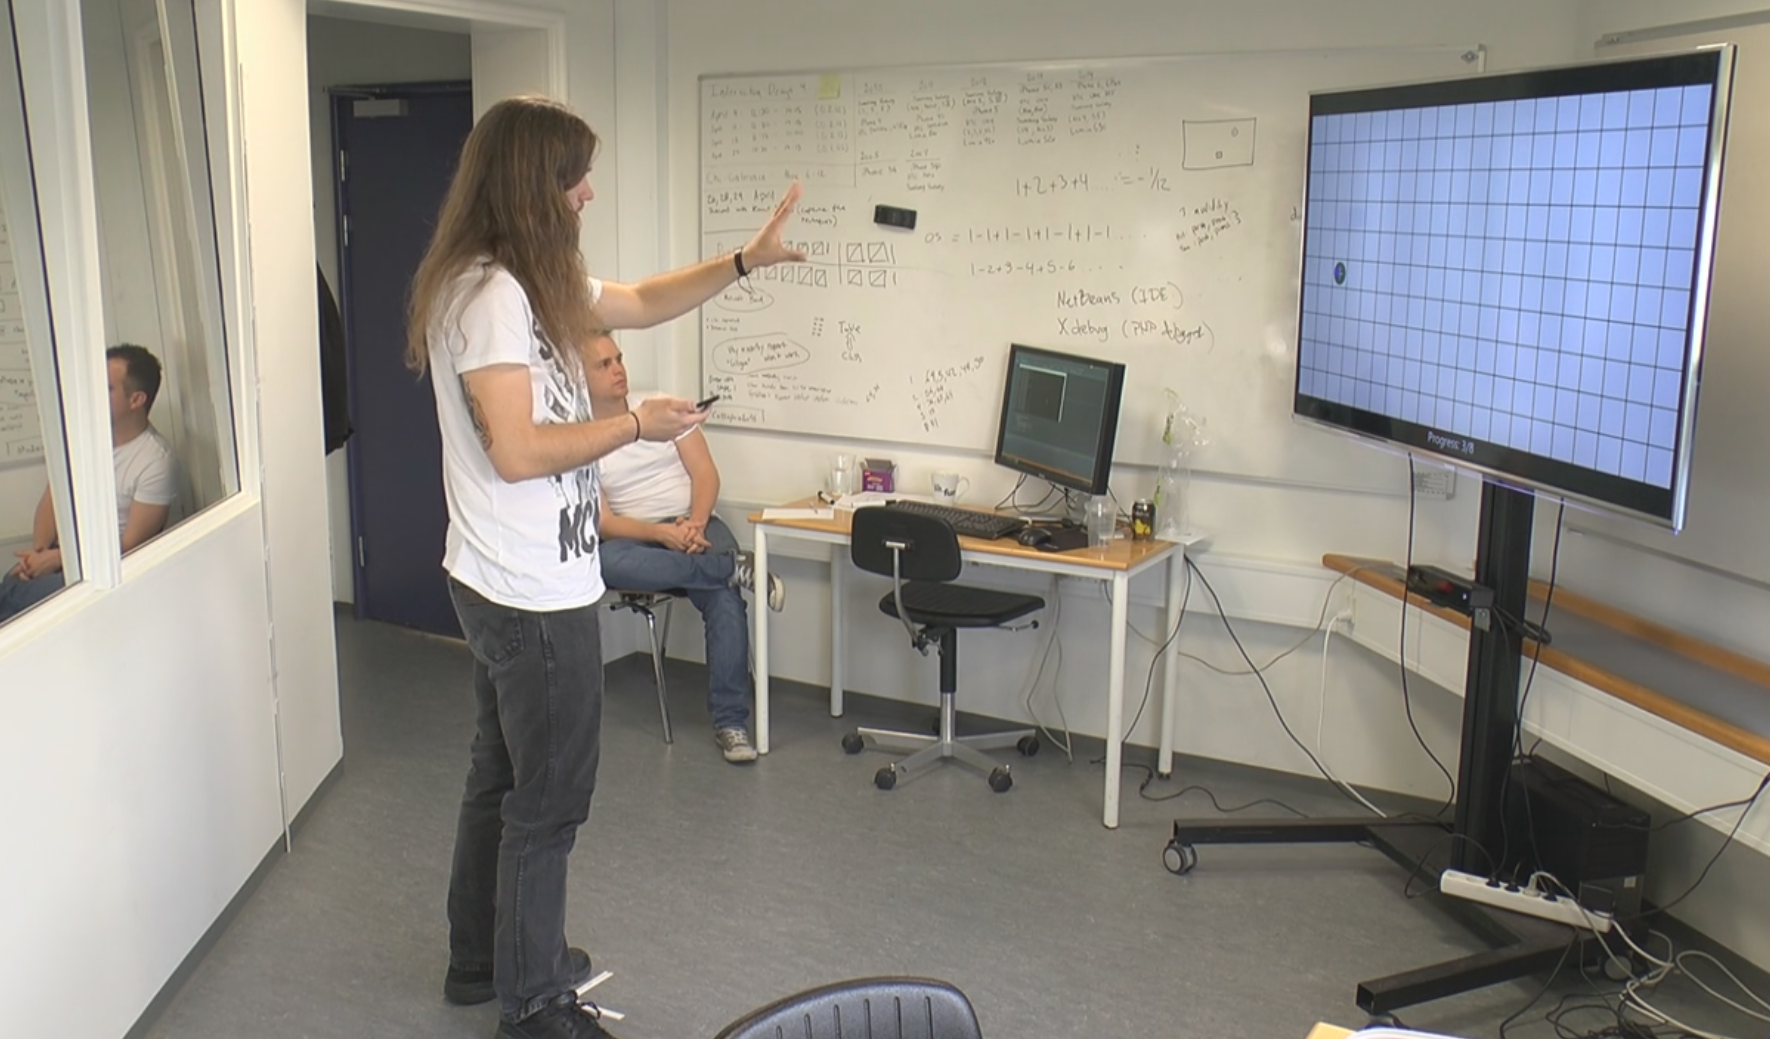
\includegraphics[width = 0.33\columnwidth]{images/accuracy.pdf}\label{fig:accuracy}}
\caption{\protect\subref{fig:target} The targets in the first part of the experiment. \protect\subref{fig:accuracy} The targets in the second part of the experiment.}
\end{figure}

Before a participant started the experiment, the general purpose of the study would be explained to the participant.
The 8 techniques were presented one technique after another and before a technique would start, a demonstration video of that technique were shown to the participants on the large display.
After two iterations of showing the video of the large screen the video runs in a loop on the smaller display.
Screenshots of the Push Throw technique demo is shown in \Cref{fig:demovideo}.

\begin{figure}[H]
\subfloat[]{\includegraphics[width = 0.5\columnwidth]{images/demovideo1.pdf}\label{fig:demovideA}}
\subfloat[]{\includegraphics[width = 0.5\columnwidth]{images/demovideo2.pdf}\label{fig:demovideB}}\\
\subfloat[]{\includegraphics[width = 0.5\columnwidth]{images/demovideo3.pdf}\label{fig:demovideC}}
\subfloat[]{\includegraphics[width = 0.5\columnwidth]{images/demovideo4.pdf}\label{fig:demovideD}}
\caption{The screen at different times during the demonstration video. The video was shown to the participant before each technique test starts. \protect\subref{fig:demovideA} Presenting the technique with the direction and the name. \protect\subref{fig:demovideB}, \protect\subref{fig:demovideC}, \protect\subref{fig:demovideD} The video pauses and the participant will be able to read the instructions on the screen.}
\label{fig:demovideo}
\end{figure}

The experiment was conducted in the usability lab at Aalborg University and in the lab we had setup a large 65 inch screen and a smaller 42 inch screen. 
A Kinect v2 was mounted below the large display.
We marked a spot on the floor with a cross where participants were asked to stand.
The setup is illustrated in \Cref{fig:setup}.

\begin{figure}[H]
\subfloat[]{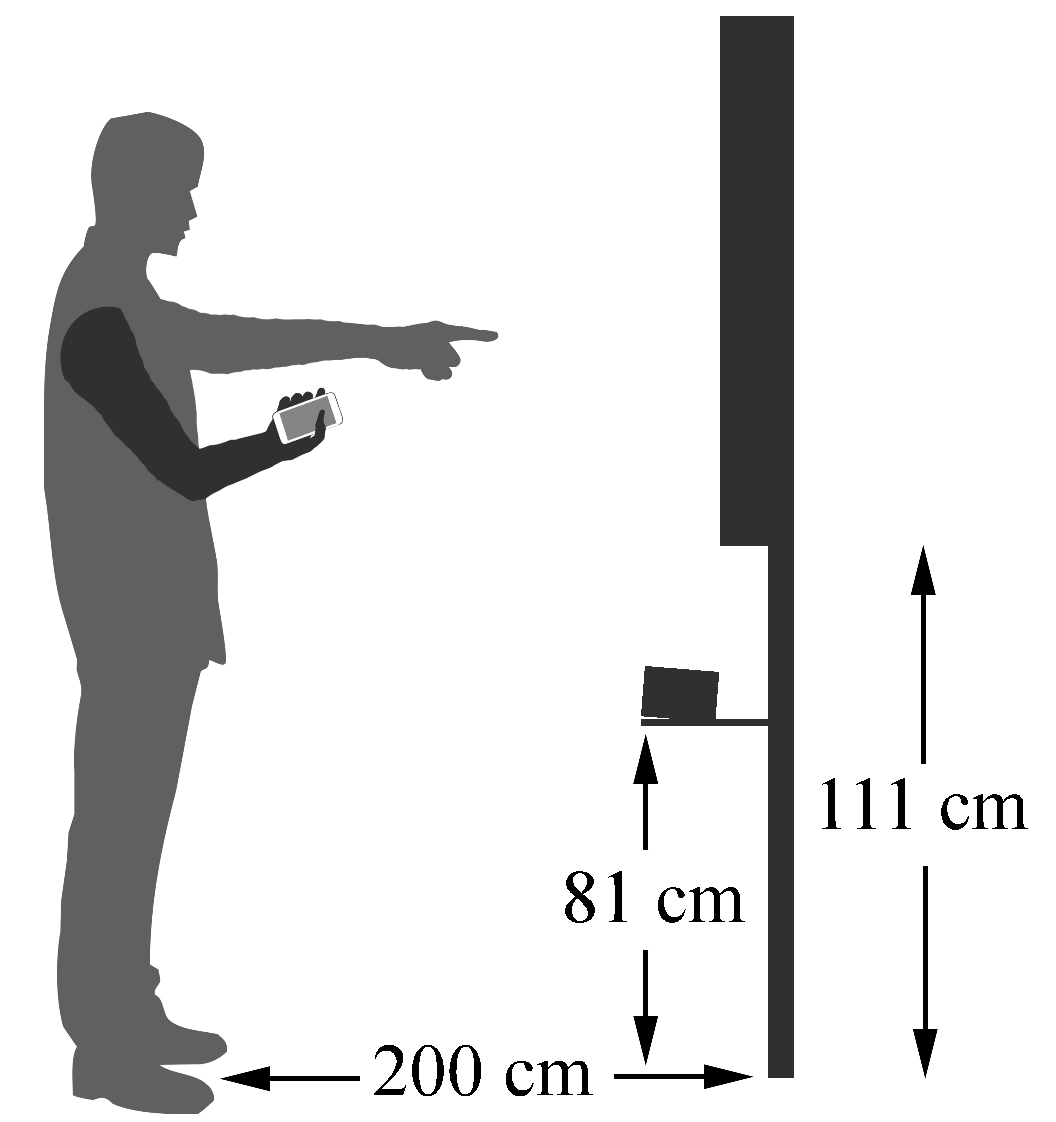
\includegraphics[width = 0.65\columnwidth]{images/setup.pdf}\label{fig:setup}}
\subfloat[]{
\includegraphics[width = 0.3\columnwidth]{images/phoneScreenshot.png}\label{fig:phoneScreen}}
\caption{\protect\subref{fig:setup} illustrates the setup and distance between participant and screen, floor and Kinect, and floor and the bottom of the large display.\protect\subref{fig:phoneScreen} shows the scrren on the phone when push techniques are used.}
\end{figure}